---
title: Cohen実数はSuslin木を付加する
date: 2016/07/08 18:08:00 JST
author: 石井大海
description: Shelahは実数の集合の性質に関する記念碑的論文において滅茶苦茶いろいろな事を示していて本当にヤバいんですが,その中で一節割いて「Cohen実数を付加するとSuslin木も足される」という事を示しています.原論文における構成は結構煩雑に見えますが,後にTodorčevićは彼の発明した\emph{minimal walk}の手法を用いて自然で比較的簡単な構成を与えました.minimal walkの手法はAronszajn木の構成にも使えますが,これとCohen実数を単に合成してやる事でSuslin木が得られるのです.本稿ではこの方法について(強制法の基礎理論は別にして)証明します.
latexmk: -lualatex
tag: 数学,数理論理学,集合論,無限組合せ論,極小歩,minimal walk,木,Suslin木,Aronszajn木,強制法,Cohen実数
---
\RequirePackage{luatex85}
\documentclass[a4j]{ltjsarticle}
\usepackage[hiragino-pron]{luatexja-preset}
\usepackage{mystyle}
\usepackage{luatexja-otf}
\usepackage{unicode-math}
\usetikzlibrary{matrix,arrows,shapes,backgrounds,positioning}
\usetikzlibrary{arrows,calc,decorations.pathmorphing}
\usetikzlibrary{decorations.markings,intersections,decorations.pathreplacing}
\setmathfont{latinmodern-math.otf}
\setmathfont{Asana Math}[range={\setminus,\models,"029F5,"022A7}]
\setmathfont{TeX Gyre Pagella Math}[range={bb}]
\setmathfont{latinmodern-math.otf}[range={up,sfup,cal}]
\setmathfont{XITS Math}[range={scr,bfscr,}]
\newcommand{\mathds}[1]{\symbb{#1}}
\usepackage{luatexja-ruby}
\renewcommand{\defeq}{\mathrel{\coloneq}}
\DeclareMathAlphabet{\mathrsfs}{U}{rsfso}{m}{n}
\renewcommand{\mathscr}[1]{\mathup{\mathrsfs{#1}}}
\usepackage{fixme}
\usepackage[bookmarksnumbered,pdfproducer={LuaLaTeX},%
            luatex,psdextra,pdfusetitle,pdfencoding=auto]{hyperref}
\usepackage[backend=biber, style=math-numeric]{biblatex}
\addbibresource{myreference.bib}
 \renewcommand{\emph}[1]{\textsf{\textgt{#1}}}

\title{Cohen実数はSuslin木を付加する}
\date{2016-07-07}
\author{石井大海}

\usepackage{amsmath}
\begin{document}

\maketitle
\begin{abstract}
 Shelahは実数の集合の性質に関する記念碑的論文~\cite{Shelah:1984}において滅茶苦茶いろいろな事を示していて本当にヤバいんですが,その中で一節割いて「Cohen実数を付加するとSuslin木も足される」という事を示しています.
 原論文における構成は結構煩雑に見えますが,後にTodor\v{c}evi\'{c}~\cite{Todorcevic:1987fj}は彼の発明した\emph{minimal walk}の手法を用いて自然で比較的簡単な構成を与えました.
 minimal walkの手法はAronszajn木の構成にも使えますが,これとCohen実数を単に合成してやる事でSuslin木が得られるのです.
 本稿ではこの方法について(強制法の基礎理論は別にして)証明します.
\end{abstract}

\section{Cohen実数はSuslin木を付加する}
念の為,木に関する\emph{木}本的な定義を復習しておく.

\begin{definition}
 \begin{itemize}
  \item $T \subseteq \power{<\alpha}{X}$が\emph{木}(\emph{tree}) $\defs$ $T$は始切片について閉じている:$\forall t \in T \: \forall n < \lh(t)\: t\restr n \in T$.
  \item $C \subseteq T$が\emph{鎖}$\defs$ $C$は$(T, \subseteq)$の全順序部分集合.
  \item $A \subseteq T$が\emph{反鎖}$\defs$任意の$s, t \in A$, $s \neq t$に対し$s \nsubseteq t$かつ$t \nsubseteq s$.
  \item $x \in T$に対し,$\rank_T(x) \defeq \sup\Set{ \rank_T(y) + 1 | y \in T, y \subsetneq x}$を$x$の$T$における\emph{ランク}と言う.
  \item $\height(T) \defeq \sup_{x \in T} (\rank_T(x) + 1)$を$T$の\emph{高さ}と呼ぶ.
  \item $T_\alpha \defeq \Set{x \in T | \rank_T(x) = \alpha}$.
  \item $T$が\emph{$\kappa$-木}$\defs$ $\height(T) = \kappa$かつ任意の$\alpha < \kappa$に対し$|T_\alpha| < \kappa$.
  \item $T$が\emph{$\kappa$-\ruby{Aronszajn}{アロンシャイン}木}$\defs$ $T$は$\kappa$-木で$T$の鎖は全て濃度$\kappa$未満.

        $\omega_1$-Aronszajn木の事を単に\emph{Aronszajn木}と呼ぶ.
  \item $T$が\emph{$\kappa$-Suslin木}(または\emph{$\kappa$-Souslin木}とも)$\defs$ $T$は$\kappa$-Aronszajn木で,$T$の任意の反鎖は濃度$\kappa$未満.

        $\omega_1$-Suslin木の事を単に\emph{Suslin木}と呼ぶ.
 \end{itemize}
\end{definition}

\begin{theorem}[Shelah~\cite{Shelah:1984}]
 Cohen強制法$\mathbf{C}$はSuslin木を付加する.
\end{theorem}

まず次の補題を認める:

\begin{lemma}
 次を満たす列$\Braket{e_\alpha | \alpha < \omega}$が存在する:
 \begin{enumerate}
  \item 単射性:各$\alpha$について$e_\alpha : \alpha \xrightarrow{\text{1-1}} \omega$,
  \item 斉一性:各$\alpha < \beta < \omega_1$に対し,$|\Set{\xi < \alpha | e_\alpha(\xi) \neq e_\beta(\xi)}| < \aleph_0$.
 \end{enumerate}
\end{lemma}

これを認めた上で先に定理1を示す.
まず,このような列からAronszajn木が作れることを見ておく:

\begin{lemma}
 補題1のような$\Braket{e_\alpha | \alpha < \omega_1}$に対し,$T \defeq \Set{e_\alpha \restr \beta | \beta \leq \alpha < \omega_1}$はAronszajn木となる.
\end{lemma}
\begin{proof}
 まず$T$が$\omega_1$-木となることを見る.
 $T$の第$\alpha$レベルは$T_\alpha \defeq \Set{ e_\beta \restr \alpha | \beta \in [\alpha, \omega_1)}$と書け,明らかに$e_\alpha \in T_\alpha$なので,$\mathop{\mathreg{ht}}(T) = \omega_1$は良い.
 また,条件(2)から$t \in T_\alpha \iff |\Set{\xi < \alpha | t(\xi) \neq e_\alpha(\xi)}| < \aleph_0$なので,結局$|T_\alpha| \leq [\alpha]^{<\aleph_0} \times \omega = \aleph_0$より$T_\alpha$は可算.
 以上より$T$は$\omega_1$-木である.

 最後に$T$が非可算鎖を持たないことを示そう.
 そこで$C \subseteq T$が非可算鎖だったとすると,共終性から$\bigcup C: \omega_1 \to \omega$となる.
 しかし,条件(1)より$C$の各元は単射なので,その貼り合わせも単射であり,$C$は$\omega_1$から$\omega$への単射となってしまうので矛盾. \qed
\end{proof}


\begin{proof}[Proof of Theorem 1]
 $V$で補題1の性質を満たす$\Braket{e_\alpha | \alpha < \omega_1}$を取り,$r$を$V$上のCohen実数とする.
 この時,$T(r) \defeq \Set{r \circ e_\alpha \restr \beta | \beta < \alpha < \omega_1}$ が$V[r]$でSuslin木となる事を示そう.

 まず,上と同様に$T_\alpha(r) = \Set{ r \circ e_\beta \restr \alpha | \beta \in [\alpha, \omega_1)}$であり,前の補題と同様にして$T(r)$が$\omega_1$-木になることが従う.

 次に$T(r)$は非可算反鎖も可算反鎖も持たないことを示そう.
 $V[r]$で$\mathcal{A} = \Set{ r \circ e_{\beta(\alpha)} \restr \alpha | \alpha < \omega_1} \in [T(r)]^{\aleph_1}$を任意に取り,これが両立する二元も両立しない二元も含むことを示せばよい.
 面倒なので,以下$t_\alpha \defeq e_{\beta(\alpha)} \restr \alpha$と書くことにする.
 そこで$X_p \defeq \Set{t_\alpha | p \Vdash^{V}_{\mathbf{C}} \quoted{\dot{r} \circ t_\alpha \in \dot{\mathcal{A}}}}$とおけば,各$p \in \mathbf{C}$について$X_p \in V$が成り立つ.
 このとき,$\Set{t_\alpha | \alpha < \omega_1} = \bigcup_{p \subset r} X_p$であり,$p \subset r$なる$p$は可算個しかないので,少なくとも一つの$X_p$は非可算となる.
 よって,最初からこの$X_p$の元に範囲を取り直せば,$\Set{t_\alpha | \alpha < \omega_1} \in V$であるとしてよい.
 条件(2)より任意の$\beta < \beta' < \omega_1$に対し$t_\beta$と$t_{\beta'} \restr \beta$は有限桁しか変わらないので,一致する範囲を表す記号を用意しておく:
 \[
  \Delta(\beta, \beta') \defeq \min\Set{ n < \omega | \forall \xi < \beta \: [t_\beta(\xi), t_{\beta'}(\xi) \geq n \implies t_\beta(\xi) = t_{\beta'}(\xi)]}.
 \]
 この記号を使えば,$\mathcal{A}$が反鎖でも鎖でもない事を示すには,以下の二つの集合がそれぞれ$\mathbf{C}$で稠密となることが示せればよい:
 \begin{align*}
  E &\defeq \Set{p \in \mathbf{C} | \exists \beta < \beta' < \omega_1 \: [p \circ t_\beta = p \circ t_{\beta'} \restr \beta, \Delta(\beta, \beta') \leq \lh(p)] },\\
  D &\defeq \Set{p \in \mathbf{C} | \exists \beta < \beta' < \omega_1 \: [p \circ t_\beta \neq p \circ t_{\beta'} \restr \beta, \Delta(\beta, \beta') \leq \lh(p)]}.
 \end{align*}
 実際,$E$が$\mathbf{C}$で稠密なら,$V[r]$において$p \subset r$で$p \in E$となるものが取れ,
 証拠となる$\beta < \beta' < \omega_1$を取れば$p \circ t_\beta = p \circ t_{\beta'} \restr \beta$であり,$\Delta(\beta, \beta') \leq \lh(p)$より$r \circ t_\beta = r \circ t_{\beta'} \restr \beta$となり,これが$\mathcal{A}$の両立する二元となる.
 同様に$D$に属す$p \subseteq r$が取れれば,証拠となる$\beta < \beta'$について$r \circ t_{\beta} \perp r \circ t_{\beta'}$となるので,これら二元は両立しない.

 あとは$E$, $D$がそれぞれ稠密となる事がわかればよい.
 そこで$p \in \power{n}{\omega}$を固定する.
 これを念頭に$X_\alpha \defeq \Set{\xi < \alpha | t_{\alpha}(\xi) < n}$と置けば,各$t_\alpha$が単射である事より有限集合となる.
 よって$\Delta$-システム補題から$Z \in [W]^{\aleph_1}$と$S \in [\omega_1]^{<\aleph_0}$で
 $\forall \set{\alpha, \alpha'} \in [Z]^2\: X_\alpha \cap X_{\alpha'} = S$となる物が取れる.
 この時,$\sup S < \omega_1$だから,各$t_\alpha \restr S$の値域が$\omega$である事に注意すれば$t_\alpha \restr S$の候補は可算個しかないので,鳩ノ巣原理から$\forall \set{\alpha, \alpha'} \in  \: t_\alpha \restr S = t_{\alpha'} \restr S$となるように$Z$を取り直せる.
 一々$Z$と書くのは面倒なので,そもそも始めから$\mathcal{A}$はこのように取れているとして以下議論を進めていく.
 そこで,$\alpha_1 < \alpha_2$なる$\alpha_1, \alpha_2 \in Z$を取り,$p$を長さ$m \defeq \Delta(\alpha_1, \alpha_2)$まで拡張する事を考えよう.

 まず$E$に属する元を取りたい.
 $k = t_{\alpha_1}(\xi) \neq t_{\alpha_2}(\xi) = \ell$となるような$k, \ell$が共に$n$以上であれば,
 $q(k) = 0$によって潰せば良い.
 もし少なくとも一方が$n$未満であれば,同じ行き先に行くように潰してやればよい.
 \[
  q(k) \defeq \begin{cases}
               p(\ell) & \exists \xi < \alpha_1 \: k = t_{\alpha_i}(\xi) \wedge \ell = t_{\alpha_{1-i}}(\xi) < n\\
               0 & \text{otherwise}.
              \end{cases}
 \]
 すると定義から$q \circ t_{\alpha_1} = q \circ t_{\alpha_2} \restr \alpha_1$であり$q \leq p$, $\lh(q) = \Delta(p, q)$である.

 最後に$D$に入るように延ばせる事を見る.
 この時,相異なる$\alpha < \alpha' \in Z$で$n \leq \Delta(\alpha, \alpha')$を満たすものが取れる.
 なぜなら,もし仮に任意の$\alpha, \alpha' \in Z$に対し$\Delta(\alpha, \alpha') < n$となるのであれば,適当な$\alpha_0 \in Z$を取って,
 \[
  e'_{\beta(\alpha)}(\xi) \defeq \begin{cases}
                                  e_{\beta(\alpha_0)}(\xi) & e_{\beta(\alpha)}(\xi) < n\\
                                  e_{\beta(\alpha)}(\xi)   & \text{otherwise}
                                 \end{cases}
 \]
 と定めてやれば,族$\Braket{e'_\alpha | \alpha < \omega_1}$は依然として仮定(1), (2)を満たす.
 しかし,この時$\Set{e'_{\beta(\alpha)} \restr \alpha | \alpha \in W}$は$\Set{e'_\alpha \restr \beta | \alpha, \beta < \omega_1}$の鎖となり,補題2に反する.
 よって,$\Delta(\alpha_0, \alpha_1) \geq n$を満たす$\alpha_0 < \alpha_1 \in W$が存在する.
 そこで$t_{\alpha_i}(\xi)$の少なくとも一方が$n$以上となるような$\xi < \beta$を取り,$m \defeq \max\set{t_{\alpha_0}(\xi), t_{\alpha_1}(\xi)}$とする.
 この時,$n \leq k \leq \Delta(\alpha_0, \alpha_1)$
 \[
  q(k) \defeq
  \begin{cases}
   p(t_{\alpha_{1-i}}(\xi)) + 1 & (t_{\alpha_i}(\xi) = k, t_{\alpha_{1-i}}(\xi) < n)\\
   k & (\ow)
 \end{cases}
 \]
 とおけば$q \circ t_\beta \neq q \circ t_{\beta'} \restr \beta$.

 以上より$D$, $E$は$\mathbf{C}$で稠密となり,$V[r] \models \quoted{T_r: \text{Suslin}}$が言えた. \qed
\end{proof}

\section{斉一列$e_\alpha$の構成}
最後に補題1を満たす$\Braket{e_\alpha | \alpha < \omega_1}$をTodor\v{c}evi\'{c}によるwalkの手法を用いて構成する.

\begin{definition}
 \begin{itemize}
  \item 以下を満たす$\Braket{C_\alpha | \alpha < \omega_1}$を\emph{$C$-列}と呼ぶ:
  \begin{enumerate}
   \item $C_{\alpha + 1} \defeq \set{\alpha}$,
   \item $C_\gamma \subseteq \gamma$ : cofinal in $\gamma$, $\otp(C_\gamma) = \omega$.
  \end{enumerate}
        $C$-列は明らかに存在するので,以下一つ固定する.
  \item $\alpha < \beta < \omega_1$に対し,$\beta$から$\alpha$への\emph{step}とは$\min(C_\beta \setminus \alpha) < \beta$の事.
  \item $\beta$から$\alpha$への\emph{walk}とは次で定まる$\Braket{s^\beta_\alpha(i) | i < \omega}$の事:
        \[
         s^{\beta,\alpha}_0 \defeq \beta,\qquad
         s^{\beta,\alpha}_{i+1} \defeq \min(C_{s^{\beta,\alpha}_i} \setminus \alpha).
        \]
        walkは順序数の真の減少列なので有限長で止まる.
        定義より$\forall i \: s^{\beta,\alpha}_i \geq \alpha$であり,$C$-列の取り方より$s^{\beta,\alpha}_i > \alpha$なら$s^{\beta,\alpha}_{i+1}$は必ず定まるので,特に最終的に$\alpha$と一致する.
  \item $\rho_1(\alpha, \alpha) = 0, \rho_1(\alpha, \beta) \defeq \max\{\ |C_\beta \cap \alpha|, \rho_1(\alpha, s^{\beta,\alpha}_1)\ \}$
        により関数$\rho_1$を定める.$\rho_1(\alpha, \beta)$を\emph{$\beta$から$\alpha$へのwalkの最大重み(maximal weight)}と呼ぶ.
 \end{itemize}
\end{definition}

定義だけだとわかりづらいと思うので,$\alpha < \beta < \omega_1$を固定しよう.
記号が重いので,$\beta_i \defeq s^{\beta,\alpha}_i$と略記することにすれば,以下のように図示出来る:
\begin{center}
 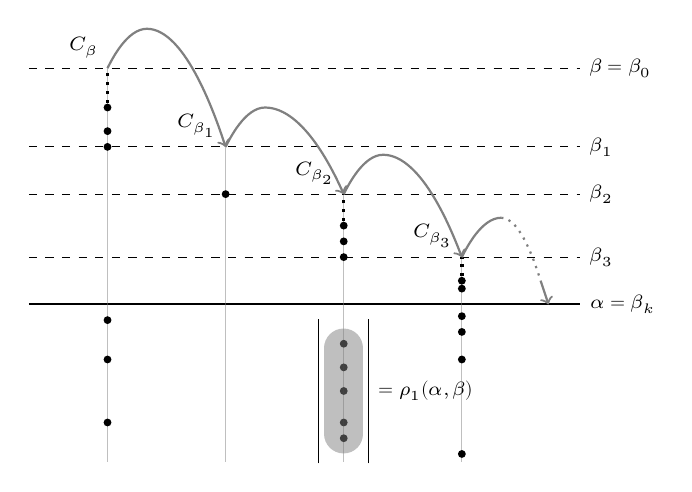
\begin{tikzpicture}[every node/.style={font=\scriptsize}]
  \path[dashed,draw] (-5, 5) -- ++ (7, 0) node[right]{$\beta = \beta_0$};
  \path[draw, thick] (-5, 2) -- ++ (7, 0) node[right]{$\alpha = \beta_k$};
  \coordinate[label=above left:{$C_\beta$}]  (s0) at (-4,5);
  \path[gray,opacity=.5,draw]
    (s0) -- (s0 |- 0, 0);

  \foreach \i/\y in {0/4 , 1/4.2, 2/4.5} {
    \node[fill=black,inner sep=1pt,circle] (C-0-\i) at (s0 |- 0, \y) {} ;
  };
  \foreach \i/\y in {0/.5 , 1/1.3, 2/1.8} {
    \node[fill=black,inner sep=1pt,circle] (W-0-\i) at (s0 |- 0, \y) {} ;
  };
  \path[dotted, draw, very thick] (C-0-2) -- (s0);

  \coordinate[label={above left:$C_{\beta_1}$}] (s1) at (C-0-0 -| -2.5,0);
  \path[dashed,draw] (-5, 0 |- s1) -- (2, 0 |- s1) node[right]{$\beta_1$};
  \path[gray,opacity=.5,draw]
    (s1) -- (s1 |- 0, 0);
  \node[fill=black, inner sep=1pt, circle]
    (C-1-0) at ($(s1)-(0,.6)$) {};

  \coordinate[label={above left:$C_{\beta_2}$}] (s2) at (C-1-0 -| -1,0);
  \path[dashed,draw] (-5, 0 |- s2) -- (2, 0 |- s2) node[right]{$\beta_2$};
  \path[gray,opacity=.5,draw]
    (s2) -- (s2 |- 0, 0);
  \foreach \i/\y in {0/2.6,1/2.8 , 2/3} {
    \node[fill=black,inner sep=1pt,circle] (C-2-\i) at (s2 |- 0, \y) {} ;
  };
  \foreach \i/\y in {0/.3 , 1/.5, 2/.9, 3/1.2, 4/1.5} {
    \node[fill=black,inner sep=1pt,circle] (W-2-\i) at (s2 |- 0, \y) {} ;
  };
  \path[dotted, draw, very thick] (C-2-2) -- (s2);

  \path[draw=gray,opacity=.5,fill=gray,line cap=round,line width=5mm]
    (W-2-0) --  (W-2-4);
  \path[draw]
    ($(W-2-0.south west)-(2.8mm,2.8mm)$) -- ($(W-2-4.north west)+(-2.8mm,2.8mm)$)
  ;
  \path[draw]
    ($(W-2-0.south east)+(2.8mm,-2.8mm)$) --
    node[right,black] {$= \rho_1(\alpha, \beta)$}
    ($(W-2-4.north east)+(2.8mm,2.8mm)$)
  ;

  \coordinate[label={above left:$C_{\beta_3}$}] (s3) at (C-2-0 -| .5,0);
  \path[dashed,draw] (-5, 0 |- s3) -- (2, 0 |- s3) node[right]{$\beta_3$};
  \path[gray,opacity=.5,draw]
    (s3) -- (s3 |- 0, 0);
  \foreach \i/\y in {0/2.2,1/2.3} {
    \node[fill=black,inner sep=1pt,circle] (C-3-\i) at (s3 |- 0, \y) {} ;
  };
  \foreach \i/\y in {0/.1 , 1/1.3, 2/1.65, 3/1.85} {
    \node[fill=black,inner sep=1pt,circle] (W-3-\i) at (s3 |- 0, \y) {} ;
  };
  \path[dotted, draw, very thick] (C-3-1) -- (s3);

  \path[draw, gray, thick, ->]
    (s0) parabola bend +(.5,.5) (s1);
  \path[draw, gray, thick, ->]
    (s1) parabola bend +(.5,.5) (s2);
  \path[draw, gray, thick, ->]
    (s2) parabola bend +(.5,.5) (s3);
  \path[draw, gray, thick]
    (s3) parabola bend ++(.5,.5) ++ (.5,.5) coordinate  (interr);
  \path[draw, dotted, gray, thick]
    (interr) parabola (1.5,2.3) coordinate (batsu);
  \path[draw, gray, thick,->]
    (batsu) -- (1.6,2);
 \end{tikzpicture}
\end{center}

$\beta$から$\alpha$に向けて$\Braket{C_\xi | \xi < \omega_1}$を梯子に使って降りていくようなイメージである.
特に,各$C_\xi$は$\omega$-型に取ってあるので,途中の$\alpha$で切ったら必ず有限で切れるようになっている.
$\rho_1$はこの$\alpha$未満の有限の端数の所に注目して,一番長い所の長さを持ってきた物である.
そして,この$\rho_1$が補題1の列を作る本質的な素になっている.

\begin{lemma}
 \begin{enumerate}
  \item $\rho_1(-, \beta)$は有限対一写像:任意の$n < \omega$に対し$|\Set{\xi < \beta | \rho_1(\xi, \beta) = n}| < \aleph_0$,
  \item $\rho_1$は斉一的(coherent):任意の$\beta < \alpha < \omega_1$に対し$|\Set{\xi < \beta | \rho_1(\xi, \beta) \neq \rho_1(\xi, \alpha)}| < \aleph_0$.
 \end{enumerate}
\end{lemma}
\begin{proof}
 \begin{enumerate}
  \item 任意の$A \in [\beta]^{\aleph_0}$と$n < \omega$に対し$n < \rho_1(\xi, \beta)$を満たす$\xi \in A$の存在を示せば良い.

        $\beta$について帰納法で示す.

        $\alpha \defeq \sup A$と置く.
        $\alpha = \beta$ならば,十分大きな$\xi \in A$で$\rho_1(\xi, \beta) \geq |C_\beta \cap \xi| > n$を満たすものがある.

        そこで$\alpha < \beta$の場合を考える.
        このとき$\alpha \leq \xi \defeq s^{\beta,\alpha}_1 < \beta$を取り,帰納法の仮定を$\xi$と$A \subseteq \xi$に適用すれば,$\eta \in A$で$n < \rho_1(\eta, \xi)$を満たすものが取れる.すると,
        \[
         \rho_1(\eta, \beta) = \max\{\ \left|C_\beta \cap \eta\right|, \rho_1(\eta, s^{\beta,\alpha}_1)\ \} > n.
        \]

        よって$\rho_1$は有限対一.
  \item $\alpha$についての帰納法で示す.

        $\beta < \alpha$と$A \in [\beta]^{\aleph_0}$を任意に取って,$\xi \in A$で$\rho_1(\xi, \beta) = \rho_1(\xi, \alpha)$を満たすものを取れれば良い.
        適切に$A$を縮めれば,$\otp A = \omega$としても一般性を失わない.
        $\gamma \defeq \sup A \leq \beta$, $\eta \defeq s^{\alpha,\gamma}_1$, $n \defeq |C_\alpha \cap \gamma|$とおく.
        上の結果から$\rho_1$は有限対一なので,
        \[
         B \defeq \Set{\xi \in A | \xi > \max(C_\alpha \cap \gamma), \rho_1(\xi, \eta) > n }
        \]
        とおけば$|A \setminus B| < \aleph_0$.
        $\xi \in B \subseteq A$をとれば,$\sup A = \gamma \geq \xi > \max(C_\alpha \cap \gamma)$より$C_\alpha \cap \xi = C_\alpha \cap \gamma$および$C_\alpha \setminus \xi = C_\alpha \setminus \gamma$.
        以上を踏まえれば,
        \begin{align*}
         \rho_1(\xi, \alpha) &= \max \{\ |C_\alpha \cap \xi|, \rho_1(\xi, s^{\alpha,\xi}_1) \ \}\\
         &= \max \{\ \underbrace{|C_\alpha \cap \gamma |}_{= n}, \underbrace{\rho_1(\xi, \eta)}_{> n} \ \} = \rho_1(\xi, \eta).
        \end{align*}
        ここで,$\eta = \beta$なら$\rho_1(\xi, \alpha) = \rho_1(\xi, \beta)$となるので適当に$\xi \in B$を取ればそれが求めるものである.
        もし$\eta < \beta$であれば,$B$に帰納法の仮定が使え,$\xi \in B$で$\rho_1(\xi, \eta) = \rho_1(\xi, \beta)$を満たすものが取れ,上の議論と合わせて$\rho_1(\xi, \alpha) = \rho_1(\xi, \beta)$となる. \qed
 \end{enumerate}
\end{proof}

\begin{proof}[Proof of Lemma 1]
 補題3より$\rho_1$は有限対一であるという所以外は条件を満たす.
 そこで,以下のように$e_\alpha$を定めれば良い:
 \[
  e_\alpha(\xi) \defeq 2^{\rho_1(\xi, \alpha)}
 \left( 2 \left|\Set{\eta \leq \xi | \rho_1(\eta, \alpha) = \rho_1(\xi, \alpha)}\right| + 1 \right).
 \]
 有限対一なので$e_\alpha$は自然数値関数としてwell-definedであり,単射なのは明らかである.
 また,$\rho_1$の斉一性より,十分大きな$n < \omega$では$\xi$のダブり方も一致するので,斉一性も成り立つ. \qed
\end{proof}

\nocite{Shelah:1984,Kunen:1980,Jech:2002}
\nocite{Bekkali:1991bv,Miyazaki:2013fv}
\printbibliography[title=参考文献]
\end{document}
